
\documentclass[fleqn,a4paper,12pt]{article}

% fleqn to left align equations
%\setlength{\textwidth}{2in}
\usepackage{hyperref}
\usepackage{fancyhdr}
\usepackage{enumitem}
%\renewcommand{\familydefault}{\rmdefault}
\renewcommand{\familydefault}{\sfdefault}
%\usepackage{helvet}
%\pagestyle{fancy}
\date{}
%\pagenumbering{gobble}
\usepackage{geometry}
\pagenumbering{gobble}
\usepackage{multicol}
\usepackage{tikz}
\usepackage{amsmath}
\usepackage{amsfonts}
\usepackage{mathtools,xparse}
\usepackage{listings}


%\fancyhf{}
%\pagestyle{fancy}
%\rhead{Mina Jafari}
%\lhead{ML-HW1}
\newcommand{\norm}[1]{\left\lVert#1\right\rVert}

%Abernethy
\newcounter{probnum}
\newcounter{subprobnum}
\newcounter{subsubprobnum}
\stepcounter{probnum}
\stepcounter{subprobnum}
\stepcounter{subsubprobnum}

\newcommand{\nsubprob}[2]{\addtolength{\leftskip}{-3em}\vspace{0em} \noindent \textbf{ \noindent #1) \stepcounter{subprobnum}} #2\par \addtolength{\leftskip}{3em}}

\def \probmargin{1.2em}
\def \probvspace{0em}

\newcommand{\nprob}[2]
{
	
	\vspace{\probvspace}
	\setcounter{subprobnum}{1}
	\setlength{\leftskip}{0em}
	\noindent \arabic{probnum}) \textbf{#1. } #2 
	\vspace{\probvspace}
	\stepcounter{probnum}
}

\newcommand{\subprob}[1]
{
	
	\setlength{\leftskip}{\probmargin}
	\setcounter{subsubprobnum}{1}
	
	\def \subttl{\textbf{(\alph{subprobnum}) }}
	\settowidth{\parindent}{\subttl}
	\addtolength{\leftskip}{\parindent}
	\setlength{\parindent}{-\parindent}
	\subttl #1
	\stepcounter{subprobnum}
	\vspace{\probvspace}
	\setlength{\parindent}{0em}
	
}

\newcommand{\subsubprob}[1]
{
	
	\setlength{\leftskip}{\probmargin}
	\addtolength{\leftskip}{\probmargin}
	
	\def \subttl{\textbf{(\roman{subsubprobnum}) }}
	\settowidth{\parindent}{\subttl}
	\addtolength{\leftskip}{\parindent}
	\setlength{\parindent}{-\parindent}
	\subttl #1
	\stepcounter{subsubprobnum}
	\vspace{\probvspace}
	\setlength{\parindent}{0em}
	
}
%end-abernethy

\geometry{a4paper,left=20mm,right=20mm,top=20mm,bottom=20mm}
%\renewcommand{\headrulewidth}{1.5 pt}

\hypersetup
{
    pdfauthor={Mina Jafari},
    pdfsubject={Homework2},
    pdftitle={MachineLearning},
    pdfkeywords={ML-HW2}
}
\linespread{1.0}

\makeatletter
\newcommand{\hwclass}[1]{\def \TVclass{#1}}
\newcommand{\hwdue}[1]{\def \TVdue{#1}}
\newcommand{\hwassignment}[1]{\def \TVassignment{#1}}
\makeatother

% Title Heading
\renewcommand{\maketitle}
{
	\begin{center}
		\newlength{\titlerulewidth}
		\def \hmwkttl{{\TVclass\, - \TVassignment}}
		\settowidth{\titlerulewidth}{\hmwkttl}
		
		\rule{\titlerulewidth}{1pt}\\[3mm]
		\hmwkttl \\[3mm]
	%	\makebox[\titlerulewidth]{\small \TVname \hspace{1em} \hfill \hfill  group member: Joshua Kammeraad} \\
		\makebox[\titlerulewidth]{\small \TVname \hspace{1em}} \\
		\makebox[\titlerulewidth]{\footnotesize {group member: Joshua Kammeraad} \hspace{1em}} \\
		\rule{\titlerulewidth}{1pt}\\[3mm]
	\end{center}
	
	\vspace{3em}
}

\def\TVname{Mina Jafari}

\hwclass{EECS 545 -- Machine Learning}
\hwdue{11:00pm 01/25/2016}
\hwassignment{Homework \#2}
\begin{document}
\maketitle	

\nprob{Question 1}{

\subprob{}{
	Including the id number in the feature set will cause a false dependence of controller output on an invalid parameter. Additionally, the id number is sorted while the data is not.

\subsubprob{}{
		\begin{figure}[!ht]
		\centering
		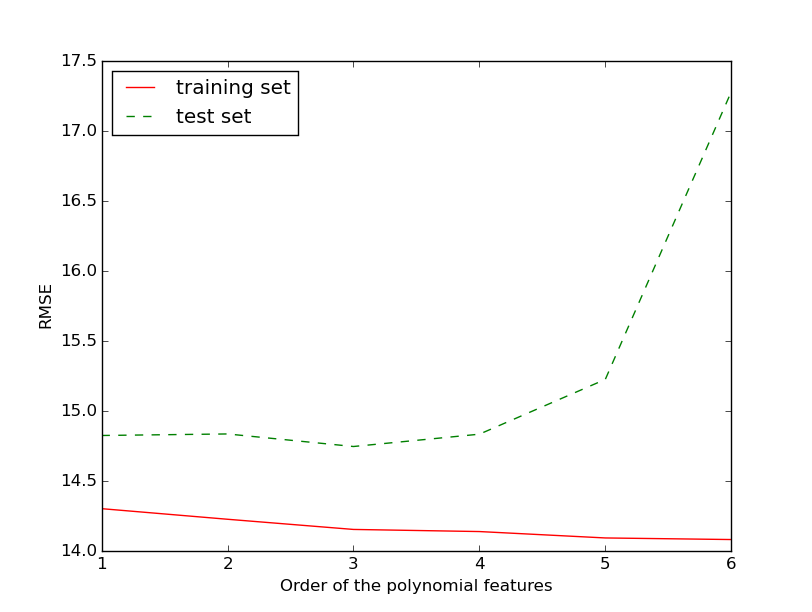
\includegraphics[width=0.5\textwidth]{question-1/1.png}
		\end{figure}
		\lstinputlisting[language=Python, basicstyle=\scriptsize]{question-1/q1-a-i.py}
}
\subsubprob{}{
			\begin{figure}[!ht]
				\centering
				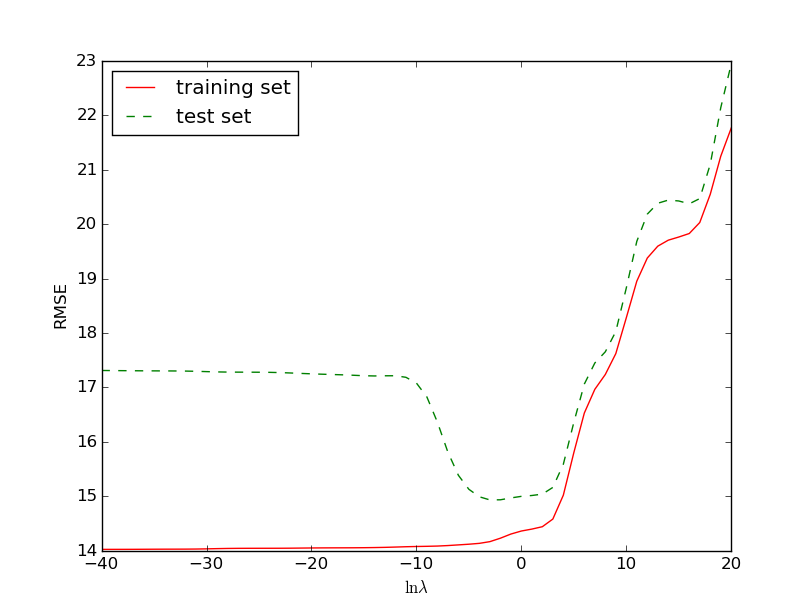
\includegraphics[width=0.5\textwidth]{question-1/2.png}
			\end{figure}
			\lstinputlisting[language=Python, basicstyle=\scriptsize]{question-1/q1-a-ii.py}
}
}	
	
\subprob{}{
		\begin{figure}[!ht]
			\centering
			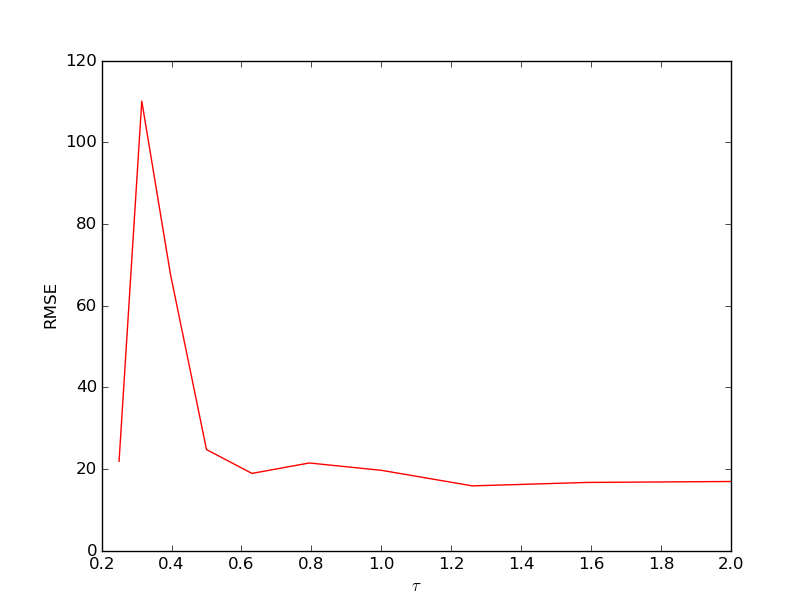
\includegraphics[width=0.5\textwidth]{question-1/3-1.png}
		\end{figure}
		\lstinputlisting[language=Python, basicstyle=\scriptsize]{question-1/q1-b.py}
}
}

\vspace{20cm}

\nprob{Question 2}{
	\lstinputlisting[language=Python, basicstyle=\scriptsize]{question-2/q2-polynomial.py}
	
	 }

\vspace{30cm}
\nprob{Question 3}{
	\subprob{}{
\begin{flalign*}
	E_D(w) &= \frac{1}{2} \sum_{i = 1}^N r_i (w^{\top} x_i - t_i)^2\\
		   &= \frac{1}{2} \sum_{i = 1}^N \big[r_i (w^{\top} x_i)^2 -2 r_i w^{\top} x_i t_i + r_i t_i^2 \big]\\
		   &= \frac{1}{2} \sum_{i = 1}^N \big[w^{\top} x_i r_i w^{\top} x_i - 2 w^{\top} x_i r_i t_i + t_i r_i t_i\big]\\
		   &= w^{\top} X^{\top} R X w - 2 w^{\top} X^{\top} R t + t^{\top} R t\\
		   &= w^{\top} X^{\top} R X w - w^{\top} X^{\top} R t - w^{\top} X^{\top} R t + t^{\top} R t\\
		   & w^{\top} X^{\top} R t = (w^{\top} X^{\top} R t)^{\top} \text{  since this is a scalar}\\
		   &= w^{\top} X^{\top} R X w - w^{\top} X^{\top} R t - t^{\top} R Xw + t^{\top} R t\\
		   &= w^{\top} X^{\top} R(X w - t) - t^{\top} R (Xw - t)\\
		   &= (w^{\top} X^{\top} - t^{\top}) (R(X w - t))\\
		   &= (Xw)^{\top} - t^{\top}) (R(X w - t))\\
		   &= (Xw - t)^{\top} R (X w - t)\\
\end{flalign*}

$\mathbf{X}$: matrix, n $\times$ m (n=number of data points in training/test set, m=number of features), each $x_i$ (data point) is one the rows of this matrix

$\mathbf{t}$: vector, n $\times$ 1 (n=number of data points in training/test set), each $t_i$ (target value) is one the elements of this vector

$\mathbf{R}$: diagonal matrix, n $\times$ n (n=number of elements in $t$), each $r_i$ (calculated weight) is one of the diagonal elements of this matrix

	}
	\subprob{}{
		\begin{flalign*}
			\nabla_w E_D(w) &= \nabla w \big((Xw - t)^{\top} R (X w - t)\big) \\
							&= \nabla w \big(w^{\top} X^{\top} R X w - 2 w^{\top} X^{\top} R t + t^{\top} R t\big)\\
							&= X^{\top} R X w - X^{\top} R t\\
			\nabla_w E_D(w^*) &= X^{\top} R X w^* - X^{\top} R t = 0\\
							& \implies w^* = (X^{\top} R X)^{-1} X^{\top} R t
		\end{flalign*}
	}
	
	\subprob{}{
	since the examples are independent, $f(t|x;w) = \prod_{i=1}^{N} p(t_i|x_i;w)$
		\begin{flalign*}
			MLE(w) &= \frac{\partial}{\partial w} {\log \bigg(\prod_{i=1}^{N} p(t_i|x_i;w)\bigg)}\\
				   &= \frac{\partial}{\partial w} {\log \bigg(\prod_{i=1}^{N} \frac{1}{\sigma_i \sqrt{2 \pi}} \exp\Big(- \frac{(t_i - w^T x_i)^2}{2 (\sigma_i)^2}\Big)\bigg)}\\
			       &= \frac{\partial}{\partial w} {\sum_{i=1}^{N} \bigg( \log \frac{1}{\sigma_i \sqrt{2\pi}} - \frac{(t_i - w^T x_i)^2}{2 (\sigma_i)^2}\bigg)}\\
			       &= \frac{\partial}{\partial w} {\sum_{i=1}^{N} \frac{-1}{2(\sigma_i)^2} (t_i - w^T x_i)^2}
		\end{flalign*}
		\begin{flalign*}
					MLE(w) &= \frac{1}{2} \frac{\partial}{\partial w} {\sum_{i=1}^{N} \frac{-1}{(\sigma_i)^2} (t_i - w^T x_i)^2}\\
				E_D(w) &= \frac{1}{2} \sum_{i = 1}^N r_i (w^{\top} x_i - t_i)^2 \implies r_i = \frac{1}{\sigma_i^2}
		\end{flalign*}
		Maximizing the likelihood function $MLE(w)$ is equivalent to minimizing its negative $-MLE(w)$, so $\frac{-1}{\sigma_i^2}$ changes to $\frac{1}{\sigma_i^2}$.
		}
	}

\vspace{30cm}
\nprob{Question 4}{
	\subprob{}{
		\lstinputlisting[language=Python, basicstyle=\scriptsize]{question-4/q4-a.py}
		\subsubprob{}{

			All of them except nominal could be used for the preprocessing, meaning we can define a median value for data of that type.\\
			The features are as follows:\\
			The first 48 columns are percentage of words in the e-mail that match a specific WORD. The next 6 columns are percentage of characters in the e-mail that match a specific character, CHAR. The following single columns are the average length of uninterrupted sequences of capital letters, length of longest uninterrupted sequence of capital letters, and sum of length of uninterrupted sequences of capital letters, respectively. The last column is a nominal {0,1} class attribute which denotes whether the e-mail was considered spam (1) or not (0).\\
			All of the feature columns can be considered ratio variables, because if their magnitude is zero, it means that word or character does not exist and the difference between two values is meaningful. However, one would argue that the difference between two values does not contain any useful information. For example, if we are trying to predict the amount of energy required to warm up a room when the outside temperature drops by 10 degrees, the magnitude of change in temperature is an important determining part of the equation. But, I am not sure if we can infer any significant information from small differences in length of capital letters or some of the other features.

			reference: \url{https://archive.ics.uci.edu/ml/datasets/Spambase}
		}
		
		\subsubprob{}{
			Test error = 25.03\% \\
			If you classify the values less than or equal to the median to be non-spam, then the error would be 10.84\%.
			
			The majority class from the training data is non-spam with 59.5\% probability. If we always predicted non-spam for the test test, the error would be 38.56\%.
		}
	}
	\subprob{}{

		The extract\_features.py script produces a sparse feature matrix with 5172 rows and 47922 columns. Given a row (data point = e-mail), value of each column is the number of times that a word appears in each e-mail. As an example, in e-mail one of the training set, the line is split after the first tab. It contains 5 words (Subject, christmas, tree, farm, pictures) and each of them occurred once. The lemmatize() function "groups together the different inflected forms of a word so they can be analyzed as a single item". The script also removes all the stopwords and punctuation marks.
		
		\lstinputlisting[language=Python, basicstyle=\scriptsize]{question-4/q4-b.py}
		}

	}
	
\vspace{30cm}	
\nprob{Question 5}{
	\subprob{}{
		\begin{flalign*}
			p(\mathbf{t}|\mathbf{w}) &= \prod_{n=1}^{N} \prod_{k=0}^{K-1} p(C_{k} | \phi(\mathbf{x}_{n}))^{\mathbf{1}(t_{n}=k)}\\
			E(\mathbf{w}) &= - \log p(\mathbf{t}|\mathbf{w}) \\
						  &= - \log \bigg(\prod_{n=1}^{N} \prod_{k=0}^{K-1} p(C_{k} | \phi(\mathbf{x}_{n}))^{\mathbf{1}(t_{n}=k)} \bigg) \\
						  &= - \log \bigg(\prod_{n=1}^{N} \prod_{k=0}^{K-1} \frac{\exp(\mathbf{w}_{k}^{T}\phi(\mathbf{x}_n))}{\sum_{k=0}^{K-1}\exp(\mathbf{w}_{k}^{T}\phi(\mathbf{x}_n))} \bigg)^{\mathbf{1}(t_{n}=k)}\\
						  &= - \sum_{n=1}^{N} \sum_{k=0}^{K-1} \mathbf{1}(t_{n}=k) \bigg[ \mathbf{w}_{k}^{T}\phi(\mathbf{x}_n) - \log \bigg( \sum_{i=0}^{K-1} \exp(\mathbf{w}_{i}^{T}\phi(\mathbf{x}_n)) \bigg)  \bigg]\\
			&\text{The above expression is non-zero only when } t_n=k \implies \\
				E(\mathbf{w}) &= - \sum_{n=1}^{N} \mathbf{w}_{t_n}^{T}\phi(\mathbf{x}_n) + \sum_{n=1}^{N} \log \bigg( \sum_{i=0}^{K-1} \exp(\mathbf{w}_{i}^{T}\phi(\mathbf{x}_n)) \bigg) \\
			&\text{Gradient of the terms where } j \neq t_n  \text{ is } 0 \text{ with respect to } \mathbf{w}_j \implies\\
			\nabla_{\mathbf{w}_j}E(\mathbf{w}) &= - \sum_{n=1}^{N} \mathbf{1}(t_{n}=j) \phi(\mathbf{x}_n) + \sum_{n=1}^{N} \bigg( \frac{\phi(\mathbf{x}_n) \exp(\mathbf{w}_{j}^{T}\phi(\mathbf{x}_n)}{\sum_{i=0}^{K-1}\exp(\mathbf{w}_{i}^{T}\phi(\mathbf{x}_n))}\bigg)\\
			& = \sum_{n=1}^{N} \bigg( \frac{\phi(\mathbf{x}_n) \exp(\mathbf{w}_{j}^{T}\phi(\mathbf{x}_n)}{\sum_{i=0}^{K-1}\exp(\mathbf{w}_{i}^{T}\phi(\mathbf{x}_n))} - \mathbf{1}(t_{n}=j)\phi(\mathbf{x}_n) \bigg)
		\end{flalign*}
		
	}
	
	\subprob{}{
		\begin{flalign*}
			E^{\lambda}(\mathbf{w}) &= E(\mathbf{w}) + \frac{\lambda}{2} \sum_{k=0}^{K-1}\mathbf{w}_{k}^{T}\mathbf{w}_{k} \\
									&= - \sum_{n=1}^{N} \sum_{k=0}^{K-1} \mathbf{1}(t_{n}=k) \bigg[ \mathbf{w}_{k}^{T}\phi(\mathbf{x}_n) - \log \bigg( \sum_{i=0}^{K-1} \exp(\mathbf{w}_{i}^{T}\mathbf{\phi(\mathbf{x}_n)}) \bigg)  \bigg] + \frac{\lambda}{2} \sum_{k=0}^{K-1}\mathbf{w}_{k}^{T}\mathbf{w}_{k} \\
 \nabla_{\mathbf{w}_j}E^{\lambda}(\mathbf{w}) &= \nabla_{\mathbf{w}_j}E(\mathbf{w}) + \nabla_{\mathbf{w}_j} \bigg( \frac{\lambda}{2} \sum_{k=0}^{K-1}\mathbf{w}_{k}^{T}\mathbf{w}_{k} \bigg)\\
									&= \sum_{n=1}^{N} \bigg( \frac{\phi(\mathbf{x}_n) \exp(\mathbf{w}_{j}^{T}\phi(\mathbf{x}_n)}{\sum_{i=0}^{K-1}\exp(\mathbf{w}_{i}^{T}\phi(\mathbf{x}_n))} - \mathbf{1}(t_{n}=j)\phi(\mathbf{x}_n) \bigg) + \lambda\mathbf{w}_{j}
		\end{flalign*}
	
	}
	}

\end{document}